\documentclass[10pt,a4paper]{article}
\usepackage[utf8]{inputenc}
\usepackage{amsthm, amsmath, mathtools, amssymb}
\usepackage[left=1.9cm,right=1.9cm,top=2.5cm,bottom=2.5cm]{geometry}
\usepackage[colorlinks,linkcolor=blue,citecolor=blue,urlcolor=blue]{hyperref}
\usepackage{standalone}
\usepackage[catalan]{babel}
\usepackage{titlesec}
\usepackage{enumitem}
\usepackage{physics}
\usepackage[hypcap=false]{caption}
\usepackage{cancel}
\titleformat{\section}
  {\normalfont\fontsize{11}{15}\bfseries}{\thesection}{1em}{}

\newcommand{\CC}{\ensuremath{\mathbb{C}}}
\newcommand{\RR}{\ensuremath{\mathbb{R}}}
\newcommand{\QQ}{\ensuremath{\mathbb{Q}}}
\newcommand{\ZZ}{\ensuremath{\mathbb{Z}}}

\newcommand{\ii}{\mathrm{i}} % imaginary unit

\DeclareDocumentCommand\partialderivative{ s o m g d() }{ 
          % Total derivative
          % s: star for \flatfrac flat derivative
          % o: optional n for nth derivative
          % m: mandatory (x in df/dx)
          % g: optional (f in df/dx)
          % d: long-form d/dx(...)
            \IfBooleanTF{#1}
            {\let\fractype\flatfrac}
            {\let\fractype\frac}
            \IfNoValueTF{#4}
            {
                \IfNoValueTF{#5}
                {\fractype{\partial \IfNoValueTF{#2}{}{^{#2}}}{\partial #3\IfNoValueTF{#2}{}{^{#2}}}}
                {\fractype{\partial \IfNoValueTF{#2}{}{^{#2}}}{\partial #3\IfNoValueTF{#2}{}{^{#2}}} \argopen(#5\argclose)}
            }
            {\fractype{\partial \IfNoValueTF{#2}{}{^{#2}} #3}{\partial #4\IfNoValueTF{#2}{}{^{#2}}}\IfValueT{#5}{(#5)}}
        } % partial differential operator

\renewcommand{\theenumi}{\textbf{\arabic{enumi}}}
\renewcommand{\theenumii}{\textbf{\alph{enumii}}}
\renewcommand{\theenumiii}{\textbf{\roman{enumiii}}}

\renewcommand{\exp}[1]{\mathrm{e}^{#1}} % exponential function
\DeclareMathOperator*{\im}{Im}
\renewcommand{\div}{\operatorname{\mathbf{div}}} % divergence
\newcommand{\vf}[1]{\boldsymbol{\mathrm{#1}}} % math style for vectors and matrices and vector-values functions (previously it was \*vb{#1} but this does not apply to greek letters)


\newtheorem{thm}{Teorema}
\newcommand{\R}{\mathbb R}
\newcommand{\RA}{\Rightarrow}
\newcommand{\ra}{\rightarrow}
\newcommand{\RL}{\Leftrightarrow}

\title{\bfseries\Large Seminari 3}

\author{Víctor Ballester, NIU: 1570866\\ Arturo Castaño, NIU: 1566489\\ Enric Garriga, NIU: 1565357}
\date{\parbox{\linewidth}{\centering
  Equacions diferencials II\endgraf
  Grau en Matemàtiques\endgraf
  Universitat Autònoma de Barcelona\endgraf
  Maig de 2022}}

\setlength{\parindent}{0pt}
\begin{document}
\selectlanguage{catalan}
\maketitle
\section*{Problema 1}
Considerem el següent sistema diferencial:
\begin{equation}\label{sist2}
  \begin{cases}
    \dot{x}=-y+x^2-y^2=:P(x,y) \\
    \dot{y}=x(1+2y)=:Q(x,y)
  \end{cases}
\end{equation}
\subsubsection*{Apartat a)}
Definim el camp $\vf{X}:=P\pdv{}{x}+Q\pdv{}{y}$. Aleshores sabem que $H(x,y)=\frac{x^2+y^2}{1+2y}$ serà una integral primera si $\vf{X}H=0$. Fent els càlculs tenim que:
\begin{align*}
  \vf{X}H=P\pdv{H}{x}+Q\pdv{H}{y} & =(-y+x^2-y^2)\frac{2x}{1+2y}+x(1+2y)\frac{2y(1+2y)-2(x^2+y^2)}{{(1+2y)}^2} \\
                                  & =(-y+x^2-y^2)\frac{2x}{1+2y}+(y+y^2-x^2)\frac{2x}{1+2y}                    \\
                                  & =0
\end{align*}
Per tant, $H$ és una integral primera del sistema.
\subsubsection*{Apartat b)}
Sabem que si $H$ és integral primera, aleshores $F:=\frac{1}{H}$ també és integral primera. Com que les corbes de nivell de $F$ ens donen òrbites (i per tant, corbes invariants) del sistema, només cal observar que la corba invariant $F=0$ és precisament $1+2y=0$. Per tant, $1+2y=0$ és invariant.
\subsubsection*{Apartat c)}
Per tal de calcular els punts crítics cal resoldre el sistema:
$$
  \begin{cases}
    -y+x^2-y^2=0 \\
    x(1+2y)=0    \\
  \end{cases}
$$
De la segona equació deduïm immediatament que $x=0$ o $y=-\frac{1}{2}$. En el primer cas, substituint el valor de la $x$ a la primera equació deduïm que $-y-y^2=0$, i per tant, $y=0$ o $y=-1$. Obtenim doncs els punts crítics $(0,0)$ i $(0,-1)$. Pel que fa al segon cas, observem que l'equació resoltant $0=-y+x^2-y^2\big|_{y=-\frac{1}{2}}=x^2+\frac{1}{4}$ no té solució en $x$ per a $x\in\RR$. Per tant, els únics punts crítics dels sistema són únicament els dos mencionats anteriorment.
Calculem ara el seu retrat de fase local. Per això necessitem calcular primer la diferencial del sistema. Tenim que $$\vf{DX}(x,y)=\begin{pmatrix}
    2x   & -1-2y \\
    1+2y & 2x
  \end{pmatrix}$$
Si avaluem aquesta matriu als dos punts crítics trobats obtenim:
\begin{align*}
  \vf{DX}(0,0)  & =\begin{pmatrix}
                     0 & -1 \\
                     1 & 0
                   \end{pmatrix}\implies \sigma(\vf{DX}(0,0))=\{\ii,-\ii\}  \\
  \vf{DX}(0,-1) & =\begin{pmatrix}
                     0  & 1 \\
                     -1 & 0
                   \end{pmatrix}\implies \sigma(\vf{DX}(0,-1))=\{\ii,-\ii\}
\end{align*}
Observem que no podem aplicar el teorema de Hartman. Però recordem que en un sistema planar d'equacions diferencials, si la diferencial en un punt crític té valors propis imaginaris purs aleshores només pot ser un centre o un focus. Però aquest segon cas no pot ser perquè el sistema admet una integral primera. Per tant, concloem que els dos punts crítics del sistema són centres.
\subsubsection*{Apartat d)}
Escrivim primer les equacions del sistema diferencial en la carta $U_1$, tenint en compte que el grau del sistema és $d=2$:
$$
  \left\{
  \begin{aligned}
    u' & =v^2\left[-uP\left(\frac{1}{v},\frac{u}{v}\right)+Q\left(\frac{1}{v},\frac{u}{v}\right)\right]=u^3+(u^2+1)v+u=:\tilde{P}(u,v) \\
    v' & =-v^3P\left(\frac{1}{v},\frac{u}{v}\right)=(u^2+uv-1)v=:\tilde{Q}(u,v)
  \end{aligned}
  \right.
$$
Si restringim les equacions a l'infinit ($v=0$), obtenim el sistema:
$$
  \left\{
  \begin{aligned}
    u' & =u^3+u \\
    v' & =0
  \end{aligned}
  \right.
$$
Ara bé, l'equació $u^3+u=0$ té una única solució real $u=0$. Per tant, amb la carta $U_1$ només obtenim un únic punt crític a l'infinit: $(0,0)$. Estudiem el seu retrat de fase local. Per això calculem la diferencial del sistema $\vf{\tilde{X}}=(\tilde{P},\tilde{Q})$:
$$\vf{D\tilde{X}}(u,v)=\begin{pmatrix}
    3u^2+2uv+1 & u^2+1     \\
    (2u+v)v    & u^2+2uv-1
  \end{pmatrix}$$
Si avaluem aquesta matriu al punt $(0,0)$ obtenim $\vf{D\tilde{X}}(0,0)=\begin{pmatrix}
    1 & 1  \\
    0 & -1
  \end{pmatrix}$, que té valors propis $\pm 1$. Per tant, pel teorema de Hartman, el punt $(0,0)$ és una sella.\\
Ara observem que com que la carta $V_1$ només canvia el signe del sistema (ja que ${(-1)}^{d-1}=-1$) tindrem que l'únic punt d'equilibri a l'infinit amb aquesta carta serà també el $(0,0)$ i el seu comportament local serà també el d'una sella. L'única cosa que canviarà és que en un cas, les separatrius de l'infinit seran atractores i en l'altra repulsores i viceversa amb l'altra separatiu.\\
Falta comprovar si els pols del disc de Poincaré són o no punts crítics. Per això cal escriure les equacions de la carta local $U_2$ i veure si l'origen $(0,0)$ és o no un punt crític amb aquesta nova carta:
$$
  \left\{
  \begin{aligned}
    u' & =v^2\left[P\left(\frac{u}{v},\frac{1}{v}\right)-uQ\left(\frac{u}{v},\frac{1}{v}\right)\right]=-u^2-(u^2+1)v-1 \\
    v' & =-v^3Q\left(\frac{u}{v},\frac{1}{v}\right)=-uv(v+2)
  \end{aligned}
  \right.
$$
Observem que l'origen no anu\lgem a simultàniament les dues equacions. Per tant, el pol nord del disc no és un punt crític. I en conseqüència tampoc ho és el pol sud, ja que les equacions del sistema diferencial en la carta $V_2$ només difereixen amb un signe, i per tant l'origen en la carta $V_2$ tampoc podrà ser punt crític.
\subsubsection*{Apartat e)}
Per tal de poder fer més fàcilment el retrat de fase al disc de Poincaré, farem primer el retrat de fase ordinari a $\RR^2$. Sabem que les òrbites del retrat de fase seran les corbes de nivell $H(x,y)=k\in\RR$ més les corbes on no està definida $H$, en aquest cas la corba invariant $1+2y=0$. Desenvolupant una mica l'expressió $H(x,y)=k$ deduïm:
\begin{equation*}
  H(x,y)=\frac{x^2+y^2}{1+2y}=k\iff x^2+y^2=k+2yk\iff x^2 + {(y-k)}^2=k+k^2
\end{equation*}
Per tant les corbes de nivell $H(x,y)=k$ són els cercles $C_k$ centrats en el punt $(0,k)$ i de radi $\sqrt{k+k^2}$. Perquè això tingui sentit cal que $k\in\RR\setminus(-1,0)$ En els valors extrems d'aquest interval ($k=0$ i $k=-1$) obtenim els dos punts crítics finits del sistema. Si això ho complementem amb la recta invariant $1+2y=0$ trobada a l'apartat b), que és on l'integral primera no està definida, ja tenim tot el retrat de fase definit perquè els cercles $C_k$ omplen tot $\RR^2$ menys justament la recta invariant en qüestió. Finalment, per tal de trobar la direcció del camp, avaluem $\vf{X}$ en els punts $(x,-1/2)$, $x\in\RR$: $\vf{X}(x,-1/2)=(x^2+1/4,0)$. Per tant, en aquests punts (que són els punts de la recta invariant del sistema) el camp és horitzontal i dirigit cap a l'eix positiu de les abscisses. Per continuïtat de les solucions respecte de les condicions inicials ja podem deduir el sentit de gir de totes les òrbites del sistema. Així doncs, obtenim el següent retrat de fase:
\begin{center}
  \begin{minipage}{\linewidth}
    \centering
    \includestandalone[mode=image|tex,width=0.5\linewidth]{Images/retrat_r2}
    \captionof{figure}{Retrat de fase del sistema diferencial a $\RR^2$}
  \end{minipage}
\end{center}
I per tant, tenint en compte que l'origen i final de la recta invariant són els punts d'equilibri de l'infinit i que el sentit de gir de les òrbites de l'infinit el podem determinar gràcies a la continuïtat de solucions respecte de condicions inicials, obtenim el següent retrat de fase al disc de Poincaré:
\begin{center}
  \begin{minipage}{\linewidth}
    \centering
    \includestandalone[mode=image|tex,width=0.5\linewidth]{Images/retrat_disk}
    \captionof{figure}{Retrat de fase del sistema diferencial al disc de Poincaré}
  \end{minipage}
\end{center}
\newpage
\section*{Problema 2}
En aquest exercici ens disposem a demostrar que el sistema
\begin{equation}\label{edo}
  \left\lbrace \begin{aligned}
    \dot{x} & =-y-2x+(3x^2+2y^2)x=P(x,y) \\
    \dot{y} & =x-2y+(3x^2+2y^2)y=Q(x,y)
  \end{aligned}\right.
\end{equation}
té al menys una òrbita periòdica.
\\Comencem per provar que l'únic punt crític del sistema és el $(0,0)$ que, en efecte, és punt d'equilibri ja que $P(0,0)=0=Q(0,0)$. Suposem que $\exists p=(x_p,y_p)\in\mathbb{R}^2$ punt crític diferent del zero per arribar a contradicció. Comencem suposant que una de les coordenades de $p$ és igual a zero. Llavors tenim dues possibilitats:
\begin{itemize}
  \item \underline{$x_p=0$}: Per ser punt crític, $p=(0,y_p)$ compleix
        $$\left\lbrace \begin{aligned}
            0 & =-y_p-\cancel{2\cdot0}+\cancel{(3\cdot0^2+2y_p^2)\cdot0}\enskip\implies y_p=0 \\
            0 & =0-2y_p+(3\cdot0^2+2y_p^2)y_p
          \end{aligned}\right.\quad \text{ és a dir } \quad p=(0,0)\enskip !!$$
  \item \underline{$y_p=0$}: Per ser punt crític, $p=(x_p,0)$ compleix
        $$\left\lbrace \begin{aligned}
            0 & =0-2x_p+(3x_p^2+2\cdot0^2)x_p                                         \\
            0 & =x_p-\cancel{2\cdot0}+\cancel{(3x_p^2+2\cdot0^2)\cdot0}\implies x_p=0
          \end{aligned}\right.\quad \text{ és a dir } \quad p=(0,0)\enskip !!$$
\end{itemize}
Per tant, amb això veiem que si $p$ és un punt d'equilibri diferent de l'origen, ambdues coordenades han de ser diferents de zero. Això ens permet dividir-les i arribar a la contradicció final. Per ser punt crític, $p=(x_p,y_p)$ compleix
$$\left\lbrace \begin{aligned}
    0 & =-y_p-2x_p+(3x_p^2+2y_p^2)x_p \\
    0 & =x_p-2y_p+(3x_p^2+2y_p^2)y_p
  \end{aligned}\right.\iff
  \left\lbrace \begin{aligned}
    y_p+2x_p & =(3x_p^2+2y_p^2)x_p \\
    2y_p-x_p & =(3x_p^2+2y_p^2)y_p
  \end{aligned}\right.\iff$$$$
  \xLeftrightarrow[y_p\neq0]{x_p\neq0}
  \left\lbrace \begin{aligned}
    \frac{y_p+2x_p}{x_p} & =(3x_p^2+2y_p^2) \\
    \frac{2y_p-x_p}{y_p} & =(3x_p^2+2y_p^2)
  \end{aligned}\right. \implies\frac{y_p+2x_p}{x_p}=\frac{2y_p-x_p}{y_p}\iff$$
$$\iff\frac{y_p}{x_p}=-\frac{x_p}{y_p}\quad!!$$
que és una contradicció ja que qualsevol nombre $a\in\mathbb{R},\enskip a\neq0$ té el mateix signe que el seu invers, $a^{-1}$. Per tant, podem concloure que l'únic punt crític del sistema és l'origen. Això serà de gran utilitat més endavant.
\\
A continuació, considerem les e\lgem ipses
\begin{equation}
  3x^2+2y^2=1\quad\text{ i }\quad 3x^2+2y^2=3
\end{equation}
Ens disposem a provar que totes les òrbites del sistema \eqref{edo} surten de la corona topològica descrita per les dues e\lgem ipses. Per a fer-ho és suficient amb estudiar el camp vectorial sobre cada una de les e\lgem ipses, i comprovar que en tot moment el vector $(P,Q)$ del camp apunta cap a l'exterior de la corona. És a dir, volem comprovar que es dona la situació de la Figura \ref{grad}:
\begin{figure}[!ht]\centering
  \begin{minipage}[c]{0.5\textwidth}\centering
    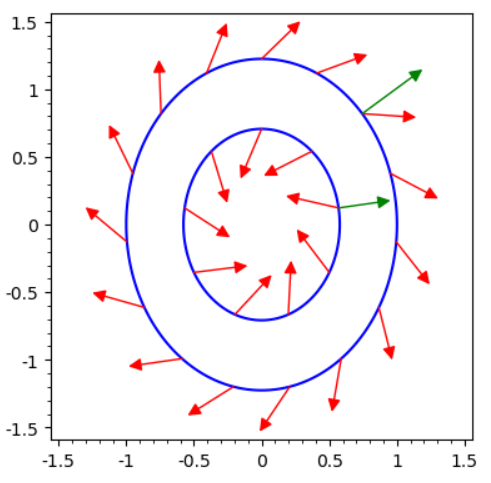
\includegraphics[scale=0.7]{Images/grad}
    \caption{Esquema no a escala del camp vectorial, on les corbes blaves són les dues e\lgem ipses, els vectors verds els seus gradients en un punt determinat i els vectors vermells representen el camp vectorial $(P,Q)$}
    \label{grad}
  \end{minipage}\hspace{0.03\textwidth}
\end{figure}
\noindent El gradient de la funció $F(x,y)=3x^2+2y^2$, això és $\nabla F=(6x,4y)$, és perpendicular a les corbes de nivell de $F$ i apunta en la direcció de creixement de la funció, en aquest cas, sempre allunyant-se de l'origen. Com les dues e\lgem ipses considerades són corbes de nivell, $\nabla F$ és un vector perpendicular a aquestes en tot punt. Per això els vectors verds de la Figura \ref{grad} representen el gradient de les corbes.
\\
És gràcies al gradient que podem esbrinar si el camp vectorial apunta cap a dins o cap enfora de la corona. Volem veure que a l'e\lgem ipse exterior es compleix $\nabla F\cdot(P,Q)>0$ --- és a dir, que l'angle entre el gradient i el vector del camp sempre serà agut --- ja que això implica que el camp vectorial surt de la corona (per a entrar a la corona, el camp vectorial com a mínim hauria de ser tangent a l'e\lgem ipse, és a dir, el producte escalar hauria de ser com a mínim zero, o negatiu si l'angle és més gran que $90^\circ$); en canvi, a l'e\lgem ipse interior succeeix el contrari i volem veure que $\nabla F\cdot(P,Q)<0$. Aleshores sabrem que tenim la situació de la Figura \ref{grad}.
\\
Comencem calculant l'expressió general del producte escalar del gradient amb el camp vectorial:
\begin{equation*}
  \begin{aligned}
    \nabla F\cdot(P,Q) & =(6x,4y)\cdot\big(-y-2x+(3x^2+2y^2)x\;,\; x-2y+(3x^2+2y^2)y\big) \\
                       & =-6xy-12x^2+6x^2(3x^2+2y^2)+4xy-8y^2+4y^2(3x^2+2y^2)             \\
                       & =-2xy-12x^2-8y^2+(6x^2+4y^2)(3x^2+2y^2)                          \\
                       & =-2xy-4(3x^2+2y^2)+2(3x^2+2y^2)^2
  \end{aligned}
\end{equation*}
I ara comprovem què passa sobre cada e\lgem ipse:
\begin{itemize}
  \item  \underline{E\lgem ipse interior}: $3x^2+2y^2=1\implies\nabla F\cdot(P,Q)=-2xy-4+2=-2(xy+1)$
        \\Ara, cal acabar d'afinar i trobar una cota per $xy$. Per això, busquem els valors màxims que poden assolir tant $|x|$ com $|y|$. Fixem-nos en que a l'expressió de l'e\lgem ipse, els termes $3x^2$ i $2y^2$ són sempre positius. Per això $x$ assolirà el seu màxim valor quan $y=0$, i viceversa. \\És a dir, en aquest cas $\displaystyle\left\lbrace
          \begin{aligned}
            |x| & \leq\frac{1}{\sqrt{3}} \\
            |y| & \leq\frac{1}{\sqrt{2}}
          \end{aligned}\right. \implies |xy|\leq\frac{1}{\sqrt{6}}\implies-\frac{1}{\sqrt{6}}\leq xy$
        \\Finalment, doncs, sobre aquesta e\lgem ipse tenim $$\nabla F\cdot(P,Q)=-2(xy+1)\leq-2\left(-\frac{1}{\sqrt{6}}+1\right)=-2\left(\frac{6-\sqrt{6}}{6} \right)<0 $$
  \item \underline{E\lgem ipse exterior}: $3x^2+2y^2=3\implies\nabla F\cdot(P,Q)=-2xy-4\cdot3+2\cdot3^2=-2(xy-3)$
        \\Repetint l'argument anterior en aquest cas tenim
        $$\displaystyle\left\lbrace
          \begin{aligned}
            |x| & \leq1                  \\
            |y| & \leq\sqrt{\frac{3}{2}}
          \end{aligned}\right. \implies |xy|\leq\sqrt{\frac{3}{2}}\implies xy\leq\sqrt{\frac{3}{2}}$$
        I per tant
        $$\nabla F\cdot(P,Q)=-2(xy-3)\geq-2\left(\sqrt{\frac{3}{2}}-3\right)=2\left(3-\sqrt{\frac{3}{2}}\right)>0 $$
\end{itemize}
Deixant així demostrat que totes les òrbites del sistema surten de la corona. El pas final, és aplicar el Teorema de Poincaré-Bendixson. Recordem-lo:
\begin{thm}
  Considerem un camp de vectors $X:\Delta\subset\mathbb{R}\longrightarrow\mathbb{R}$. Sigui $\varphi(t)=\varphi(t,p)$ la solució del camp $X$ tal que $\varphi(0,p)=p$, on $p\in\Delta$ és una condició inicial.
  \\Suposem que $\gamma_p^{-}=\left\lbrace \varphi(t)|t\leq0\right\rbrace \subset$ compacte $K\subset\Delta$, i que $X$ té un nombre finit de punts d'equilibri.
  \\Llavors es verifica una de les tres condicions següents:
  \begin{enumerate}[label=\roman*)]
    \item $\alpha(p)$ és una òrbita periòdica i tots els punts de $\alpha(p)$ són regulars.
    \item $\alpha(p)$ està format per punts d'equilibri i per òrbites que tenen els seus $\alpha$-límits i $\omega$-límits en aquests punts d'equilibri.
    \item $\alpha(p)$ és un punt d'equilibri.
  \end{enumerate}
\end{thm}
\noindent En aquest cas, la corona definida per les e\lgem ipses --- anomenem-la $K$ --- és un compacte. A més a més, gràcies al resultat que acabem de veure sobre el producte escalar $\nabla F\cdot(P,Q)$ deduïm una cosa més: Com que tots els vectors del camp apunten cap a l'exterior de la corona sobre la seva frontera, les òrbites $\varphi_p(t)$, que són tangents al camp, només poden sortir de $K$ en temps positius $\forall p \in K$. En cas contrari, si suposem que $\exists t_0<0$ tal que $\varphi_p(t_0)\notin K$, en algun moment l'òrbita hauria travessat la frontera en direcció cap a l'interior (ja que $\varphi_p(0)=p\in K$, per tant l'òrbita ha d'entrar-hi per passar per $p$) implicant que un vector del camp $X$ apunta cap a l'interior de la corona, cosa que ja hem demostrat que és falsa. Per tant, podem concloure que $\gamma_p^{-}\subset K\enskip\forall p\in K$. Finalment, com que el sistema té un nombre finit de punts d'equilibri, comprovem que es compleixen totes les hipòtesi del Teorema i podem aplicar-lo.
\\Observem que només és possible el cas $i)$ del Teorema, és a dir, que l'$\alpha$-límit de les òrbites sigui una òrbita periòdica, ja que els altres dos casos involucren que l'$\alpha$-límit contingui punts crítics diferents de l'origen (atès que l'origen no es troba dins de $K$). Així doncs, queda demostrat que el sistema ha de contenir com a mínim una òrbita periòdica, finalitzant l'exercici.



%	a més a més sabem que no es pot donar ni el cas  ni el 2 ja que a l'interior de la corona no hi ha cap punt crític, atès que l'únic del sistema es troba a l'origen. Així doncs, això implica que l'$\alpha$-límit és necessàriament una (com a mínim) òrbita periòdica que es troba a l'interior de la corona, acabant així la demostració de que el sistema ha de tenir alguna òrbita periòdica.
\newpage
\section*{Problema 3}
Considerem el sistema diferencial:
\begin{equation}
  \begin{cases}
    \dot{x}=-y(2y+1)-(x^2+y^2-1)=:P(x,y) \\
    \dot{y}=x(2y+1) =:Q(x,y)
  \end{cases}
\end{equation}
\subsection*{Apartat a)}
Definim les corbes:
$$
  f_1=\{(x,y) \mid \ 2y+1=0\}, \ \ \ \ \ f_2=\{(x,y) \mid \ x^2+y^2-1=0\}
$$
on per simplificar notació escriurem simplement $f_1(x,y)=2y+1=0$ i $f_2(x,y)=x^2+y^2-1=0$. Vegem que aquestes dues corbes són invariants:
\begin{equation}
  \frac{\partial f_1}{\partial x}P+\frac{\partial f_1}{\partial y}Q=0\cdot P+2\cdot Q=2x(2y+1)=K_1(x,y)\cdot f_1(x,y), \ \ \ K_1(x,y):=2x
\end{equation}
Fixem-nos que també podriem haver vist que aquesta recta és invariant per el següent fet: $2y+1=0 \iff y=\frac{-1}{2}$. Ara bé, per aquesta recta tindrem que $\dot{y}=0$, això és, que la coordenada $y$ no varia. Per tant, l'òrbita de qualsevol punt tal que la seva segona coordenada sigui $\frac{-1}{2}$ es mantindrà dins de la recta $y=\frac{-1}{2}$, essent per tant invariant.
\par
Per la corba $f_2$:
\begin{equation}
  \frac{\partial f_2}{\partial x}P+\frac{\partial f_2}{\partial y}Q= -2x(x^2+3y^2+y-1)+2yx(2y+1)=  -2x(x^2+3y^2+y-1-2y^2-y)
\end{equation}
$$= -2x(x^2+y^2-1)=K_2(x,y)f_2(x, y), \ \ \ K_2(x,y):=-2x$$
Per tant, la corba $f_2$ també és invariant.

\subsection*{Apartat b)}
Recordem la primera part del teorema d'integrabilitat de Darboux:
\begin{thm}
  Sigui $\dot{x}=P(x,y), \ \dot{y}=Q(x,y)$ un sistema diferencial polinomial de grau $d=\max\{\deg(P), \ \deg(Q)\}$. Siguin $f_i(x,y)=0, \ i\in\{1, 2, ..., p\}$ corbes invariants amb cofactors $K_i(x,y)$ respectivament. Siguin $e^{\frac{g_j(x,y)}{h_j(x,y)}}, \ j\in\{1, 2, ... q\}$ factors exponencials amb cofactors $L_j(x,y)$. \\
  Aleshores, si $\exists \lambda_i, \ \mu_j \in \R$ no tots nuls tals que $\sum_{i=1}^{p}\lambda_iK_i(x,y)+\sum_{j=1}^{q}\mu_jL_j(x,y)=0 \ \forall (x,y)$
  \\ $\implies H=f_1(x,y)^{\lambda_1}...f_p(x,y)^{\lambda_p}e^{\mu_1\frac{g_1(x,y)}{h_1(x,y)}}...e^{\mu_q\frac{g_q(x,y)}{h_q(x,y)}}$ és una integral primera del sistema.
\end{thm}

En el nostre cas tenim $d=2$ i, per l'apartat anterior, els cofactors són $K_1(x,y)=2x$ i $K_2(x,y)=-2x$. Llavors, fixem-nos que $K_1(x,y)+K_2(x,y)=0, \ \forall (x,y)$, i per tant aplicant el teorema de integrabilitat de Darboux deduïm que $H(x,y)=(2y+1)(x^2+y^2-1)$ és una integral primera. En efecte, comprovem-ho:
$$\frac{\partial H}{\partial x}P+\frac{\partial H}{\partial y}Q=-2x(2y+1)[y(2y+1)+(x^2+y^2-1)]+x(2y+1)[2x^2+6y^2-2+2y]$$
$$
  =2x(2y+1)[x^2+3y^2+y-1-(x^2+3y^2+y-1)]=0$$
\subsection*{Apartat c)}
Com ja vam veure al primer seminari, els sistemes hamiltonians no poden tenir ni cicles límits ni focus. Fixem-nos en el següent fet: si considerem la funció $G(x,y)=\frac{H(x,y)}{2}$:
\begin{equation}
  \begin{cases}
    \frac{-\partial G}{\partial y}=-y(2y+1)-(x^2+y^2-1)=\dot{x} \\
    \frac{\partial G}{\partial x}=x(2y+1)=\dot{y}
  \end{cases}
\end{equation}
És a dir, la funció $G(x,y)$ és un hamiltonià, i per tant per el primer seminari deduïm que aquest sistema no pot tenir cicles límits.
\par
Ara bé, el mateix argument utilitzat el primer seminari per els sistemes hamiltonians també és vàlid per sistemes amb integrals primeres, i per tant els sistemes amb integrals primeres tampoc poden tenir òrbites periòdiques. Aleshores, aplicant directament l'apartat (b) deduïm, sense haver de passar per la funció $G(x,y)$, que el sistema no pot tenir òrbites periòdiques.
\end{document}
